%%%%%%%%%%%%%%%%%%%%%%%%%%%%%%%%%%%%%%%%%%%%%%%%
% E.Pinault-Bigeard - e.pinault-bigeard@upsti.fr
% http://s2i.pinault-bigeard.com
% CC BY-NC-SA 2.0 FR - http://creativecommons.org/licenses/by-nc-sa/2.0/fr/
%%%%%%%%%%%%%%%%%%%%%%%%%%%%%%%%%%%%%%%%%%%%%%%%
\documentclass[11pt]{article}
%%%%%%%%%%%%%%%%%%%%%%%%%%%%%%%%%%%%%%%%%%%%%%%%
% Package UPSTI_Document
%%%%%%%%%%%%%%%%%%%%%%%%%%%%%%%%%%%%%%%%%%%%%%%%
%%%%%%%%%%%%%%%%%%%%%%%%%%%%%%%%%%%%%%%%%%%%%%%%
% Package UPSTI_Document
%%%%%%%%%%%%%%%%%%%%%%%%%%%%%%%%%%%%%%%%%%%%%%%%
\usepackage{subcaption}
\usepackage[usenames, svgnames, dvipsnames]{xcolor}
\usepackage{UPSTI_Document}
\usepackage{pgfplots}
\usepackage{import}
\definecolor{darkspringgreen}{rgb}{0.09, 0.45, 0.27}

\newcommandx*{\dessinRepereFigGeo}[5][1=\vx{},2=\vy{},3=\vz{},4=,5=0]
	{
		\draw [->,very thick] (0,0) -- (1,0) ;
		\draw [->,very thick] (0,0) -- (0,1) ;
    \fill[white] (0,0) circle (0.13);
    \draw [->,very thick] (0,0) circle (0.13);
    \ifnumequal{#5}{0} {% z vers nous
      \fill[black] (0,0) circle (0.03);
      \draw [->,thick] (0,0) circle (0.04);
    }{% z vers la feuille
  		\begin{scope} [rotate=45]
  			\draw [-,thick] (0,-0.12) -- (0,0.12) ;
  			\draw [-,thick] (-0.12,0) -- (0.12,0) ;
  		\end{scope}
    }
		\draw [anchor=north west] (1.1,0) node {${#1}$};
		\draw [anchor=south west] (0,1.1) node {${#2}$};
		\draw [anchor=north east] (-0.1,0) node {${#3}$};
		\draw [anchor=north west] (-0.1,-0.1) node {${#4}$};
	}

	\usepackage{array}
	\newcolumntype{L}[1]{>{\raggedright\let\newline\\\arraybackslash\hspace{0pt}}m{#1}}
	\newcolumntype{C}[1]{>{\centering\let\newline\\\arraybackslash\hspace{0pt}}m{#1}}
	\newcolumntype{R}[1]{>{\raggedleft\let\newline\\\arraybackslash\hspace{0pt}}m{#1}}

	\usepackage{pifont}% http://ctan.org/pkg/pifont
\newcommand{\cmark}{\color{green}\ding{51}}%
\newcommand{\xmark}{\color{red}\ding{55}}%
\newcommand{\fmark}{\ding{229}}%
\newcommand{\itemc}{\item[\cmark]}%
\newcommand{\itemx}{\item[\xmark]}%
\newcommand{\itemf}{\item[\fmark]}%


%---------------------------------%
% Paramètres du package
%---------------------------------%

% Version du document (pour la compilation)
% 1: Document prof
% 2: Document élève
% 3: Document à publier
\newcommand{\UPSTIidVersionDocument}{2}


% Variante
%\newcommand{\UPSTIvariante}{2}

% Classe
% 1: PTSI				6: PSI*			11: TSI2		16: Spé
% 2: PT	(par défaut)	7: MPSI			12: ATS
% 3: PT*				8: MP			13: PC
% 4: PCSI				9: MP*			14: PC*
% 5: PSI				10: TSI1		15: Sup
%\newcommand{\UPSTIidClasse}{2}



% Matière
% 1: S2I (par défaut)    2: IPT     3: TIPE
% 6: Vie au lycée
\newcommand{\UPSTIvariante}{5}
\newcommand{\UPSTIidMatiere}{0}
\newcommand{\UPSTIintituleMatiere}{Automatique}
\newcommand{\UPSTIsigleMatiere}{Autom}
% Type de document
% 0: Custom*				7: Fiche Métho de			14: Document Réponses
% 1: Cours (par défaut)		8: Fiche Synthèse    		15: Programme de colle
% 2: TD     				9: Formulaire
% 3: TP						10: Memo
% 4: Colle					11: Dossier Technique
% 5: DS						12: Dossier Ressource
% 6: DM						13: Concours Blanc
% * Si on met la valeur 0, il faut décommenter la ligne suivante:
%\newcommand{\UPSTItypeDocument}{Custom}
\newcommand{\UPSTIidTypeDocument}{1}

% Titre dans l'en-tête


% Titre dans l'en-tête

\newcommand{\UPSTIvariante}{5}

\newcommand{\UPSTItitreEnTete}{Automatisme industriel}
%\newcommand{\UPSTItitreEnTetePages}{}
\newcommand{\UPSTIsousTitreEnTete}{Introduction aux API}


% Titre
%\newcommand{\UPSTItitrePreambule}{Automatisme industriel}
\newcommand{\UPSTItitre}{La programmation d'un Automate Industriel}

% Durée de l'activité (pour DS, DM et TP)
\newcommand{\UPSTIduree}{3h30}

% Note de bas de première page
%\newcommand{\UPSTInoteBasDePremierePage}{Geoffrey Vaquette}
% Numéro (ajoute " n°1" après DS ou DM)
\newcommand{\UPSTInumero}{2}

% Numéro chapitre
%\newcommand{\UPSTInumeroChapitre}{1}

% En-tête customisé
%\newcommand{\UPSTIenTetePrincipalCustom}{UPSTIenTetePrincipalCustom}

% Message sous le titre
%\newcommand{\UPSTImessage}{Message sous le titre}


\RequirePackage[cache=false]{minted}


% Référence au programme
%\newcommand{\UPSTIprogramme}{\EPBComp \EPBCompP{B1-02}, \EPBCompP{B2-49}, \EPBCompS{B2-50}, \EPBCompS{B2-51}, \EPBCompP{C1-07}, \EPBCompP{C1-08}}

% Si l'auteur n'est pas l'auteur par défaut
%\renewcommand{\UPSTIauteur}{WWOOOOOOWW}

% Si le document est réalisé au nom de l'équipe
%\newcommand{\UPSTIdocumentCollegial}{1}

% Source
%\newcommand{\UPSTIsource}{UPSTI}

% Version du document
\newcommand{\UPSTInumeroVersion}{1.0}

%-----------------------------------------------
\UPSTIcompileVars		% "Compile" les variables
%%%%%%%%%%%%%%%%%%%%%%%%%%%%%%%%%%%%%%%%%%%%%%%%

\include{dirtree}
%%%%%%%%%%%%%%%%%%%%%%%%%%%%%%%%%%%%%%%%%%%%%%%%
% Début du document
%%%%%%%%%%%%%%%%%%%%%%%%%%%%%%%%%%%%%%%%%%%%%%%%
\usepackage{grafcet}

\usetikzlibrary[circuits.plc.ladder]            %     
\newlength{\ladderskip}\setlength{\ladderskip}{5\tikzcircuitssizeunit}%5\tikzcircuitssizeunit    = 355pt
\newlength{\ladderrungsep}
\setlength{\ladderrungsep}{.2\ladderskip}
\def\ladderrungend#1{\pgftransformyshift{-#1\ladderskip-\ladderrungsep}}


\begin{document}
\UPSTIbuildPage

%\tableofcontents

\section{Unity Pro}
\subsection{Téléchargement}
	Afin de réaliser ce TP, vous devez télécharger et installer UnityPro sur votre ordinateur.

	Ce fichier est disponible sur le lien suivant : \url{
https://www.dropbox.com/sh/swx955v2w91w0ua/AAC5ps8t7uz9rY4cHxClXFura?dl=0}

La page vous demandera un mot de passe. Le mot de passe est le suivant

\begin{description}
	\item [Lien de téléchargement : ] \url{
https://www.dropbox.com/sh/swx955v2w91w0ua/AAC5ps8t7uz9rY4cHxClXFura?dl=0}
	\item [Mot de passe : ] automatismes
\end{description}


\subsection{Installation}
Décompressez l'archive et les sous-archives que vous aurez alors téléchargées.

Ouvrez l'ISO puis double-cliquez sur \textit{setup.exe}

Durant l'installation, il vous sera demandé des informations sur le produit (Fiigure~\ref{fig:refNum}) :
\begin{description}
	\item [Num Produit : ]UNYSPUEEFV1X
	\item [Numéro de série : ] 21140211496
\end{description}

\begin{figure}[h!t]
\centering
	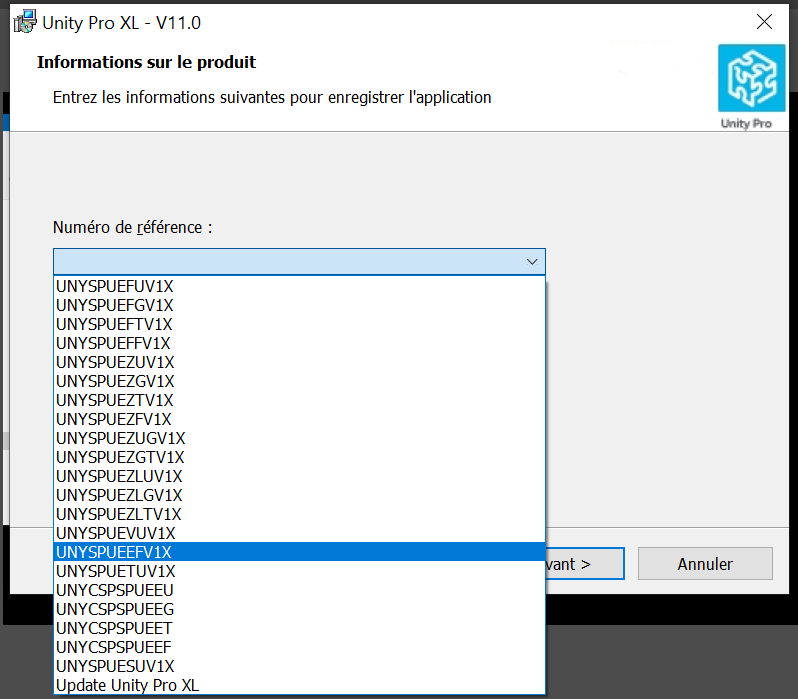
\includegraphics[width=.5\textwidth]{images/installationUnity/installNumProduit}
	\caption{Numéro de référence}
	\label{fig:refNum}
\end{figure}

L'installation dure alors quelques minutes.

\subsection{Enregistrement}
Une fois l'installation terminée, lancez le logiciel. Une fenêtre s'ouvre vous informant que votre produit n'est pas enregistré et vous demande si vous voulez l'enregistrer maintenant. Cliquez sur \textbf{Oui}, sélectionnez \textbf{Saisir le code d'autorisation reçu} puis cliquez sur Suivant et Suivant. Vous pouvez alors rentrer le code d'autorisation reçu. La Figure~\ref{fig:enregistrement} vous montre les différentes fenêtre pour l'enregistrement.

\begin{description}
	\item [Code d'autorisation : ] 52267224
\end{description}

\begin{figure}[h!t]
	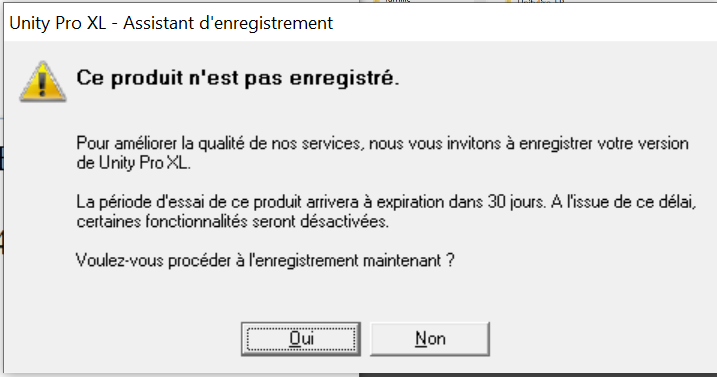
\includegraphics[width=.45\textwidth]{images/installationUnity/enregistrement}%
	\hfill 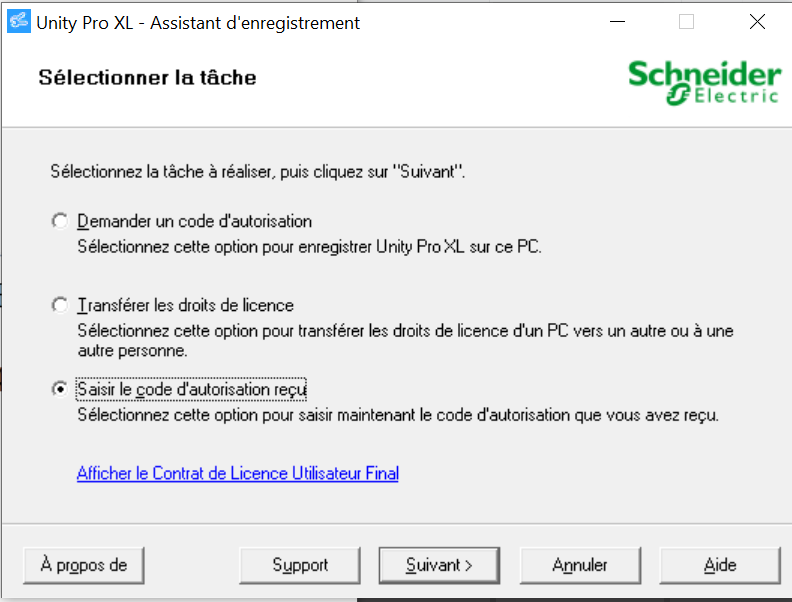
\includegraphics[width=.45\textwidth]{images/installationUnity/enregistrement-2}

\vspace{1cm}
	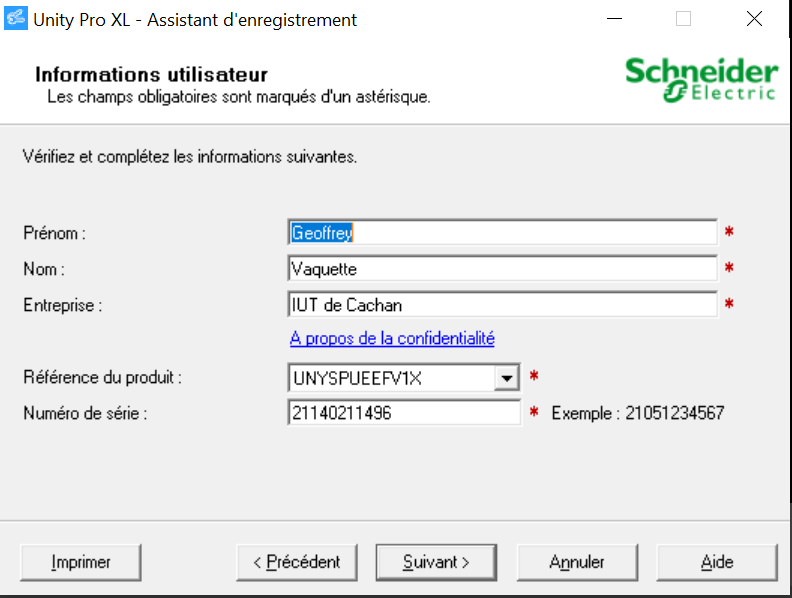
\includegraphics[width=.45\textwidth]{images/installationUnity/enregistrement-3}%
	\hfill 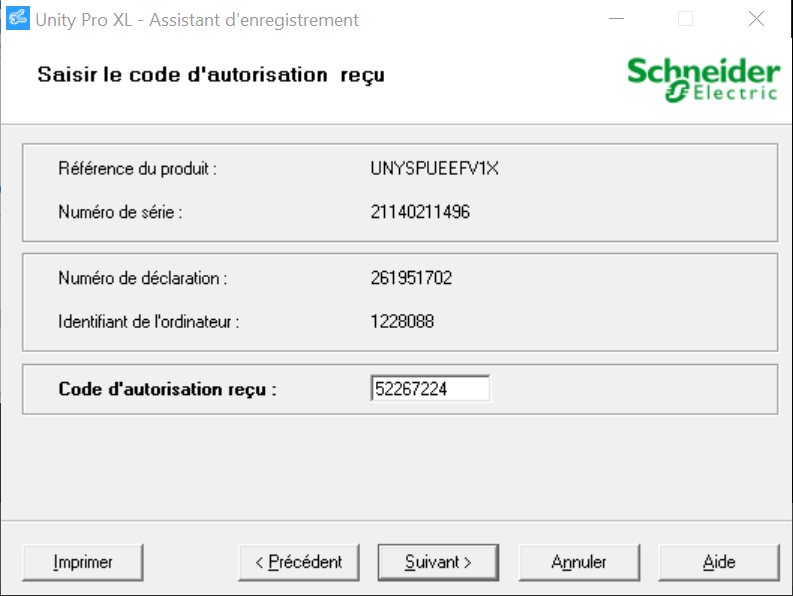
\includegraphics[width=.45\textwidth]{images/installationUnity/enregistrement-4}
	\caption{Procédure d'enrgistrement}
	\label{fig:enregistrement}
\end{figure}

\pagebreak
\section{Travail demandé}
Cette séance de travaux pratiques porte sur un système de tri de pièce. Il s'agit du même système que celui du sujet du TD n°3.
À la fin de la première séance, vous devez avoir implémenté les deux premiers cahier des charges.

Vous avez un total de deux séances pour compléter \textbf{entièrement} le TP disponible en ligne : \url{http://public.iutenligne.net/informatique/informatique-industrielle/deprez_maillefert/Autom/3TriPieces/}

\subsection{Présentation de la page en ligne}
Après avoir cliqué sur ce \href{http://public.iutenligne.net/informatique/informatique-industrielle/deprez_maillefert/Autom/3TriPieces/}{lien}, vous devriez obtenir la page suivante :

\begin{figure}[h]
\includegraphics[width=.8\textwidth]{images/triDePieceIutEnLigne/accueil}
	\caption{Page d'accueil du TP}
\end{figure}

Vous pouvez cliquer sur \textbf{suivant} en bas de la page pour passer à la page suivante
\end{document}
